\documentclass[../Main.tex]{subfiles}
\usepackage{tikz}
\usetikzlibrary{shapes.multipart}
\usetikzlibrary{positioning}
\usetikzlibrary{shadows}
\usetikzlibrary{calc}

\pgfarrowsdeclare{crow's foot}{crow's foot}
{
    \pgfarrowsleftextend{+-.5\pgflinewidth}%
    \pgfarrowsrightextend{+.5\pgflinewidth}%
}
{
    \pgfutil@tempdima=0.6pt%
    \pgfsetdash{}{+0pt}%
    \pgfsetmiterjoin%
    \pgfpathmoveto{\pgfqpoint{0pt}{-9\pgfutil@tempdima}}%
    \pgfpathlineto{\pgfqpoint{-13\pgfutil@tempdima}{0pt}}%
    \pgfpathlineto{\pgfqpoint{0pt}{9\pgfutil@tempdima}}%
    \pgfpathmoveto{\pgfqpoint{0\pgfutil@tempdima}{0\pgfutil@tempdima}}%
    \pgfpathmoveto{\pgfqpoint{-8pt}{-6pt}}% 
    \pgfpathlineto{\pgfqpoint{-8pt}{-6pt}}%  
    \pgfpathlineto{\pgfqpoint{-8pt}{6pt}}% 
    \pgfusepathqstroke%
}

\pgfarrowsdeclare{omany}{omany}
{
    \pgfarrowsleftextend{+-.5\pgflinewidth}%
    \pgfarrowsrightextend{+.5\pgflinewidth}%
}
{
    \pgfutil@tempdima=0.6pt%
    \pgfsetdash{}{+0pt}%
    \pgfsetmiterjoin%
    \pgfpathmoveto{\pgfqpoint{0pt}{-9\pgfutil@tempdima}}%
    \pgfpathlineto{\pgfqpoint{-13\pgfutil@tempdima}{0pt}}%
    \pgfpathlineto{\pgfqpoint{0pt}{9\pgfutil@tempdima}}%
    \pgfpathmoveto{\pgfqpoint{0\pgfutil@tempdima}{0\pgfutil@tempdima}}%  
    \pgfpathmoveto{\pgfqpoint{0\pgfutil@tempdima}{0\pgfutil@tempdima}}%
    \pgfpathmoveto{\pgfqpoint{-6pt}{-6pt}}% 
    \pgfpathcircle{\pgfpoint{-15.5pt}{0}} {3.5pt}
    \pgfusepathqstroke%
}

\pgfarrowsdeclare{one}{one}
{
    \pgfarrowsleftextend{+-.5\pgflinewidth}%
    \pgfarrowsrightextend{+.5\pgflinewidth}%
}
{
    \pgfutil@tempdima=0.6pt%
    \pgfsetdash{}{+0pt}%
    \pgfsetmiterjoin%
    \pgfpathmoveto{\pgfqpoint{0\pgfutil@tempdima}{0\pgfutil@tempdima}}%
    \pgfpathmoveto{\pgfqpoint{-6pt}{-6pt}}% 
    \pgfpathlineto{\pgfqpoint{-6pt}{-6pt}}%  
    \pgfpathlineto{\pgfqpoint{-6pt}{6pt}}% 
    \pgfpathmoveto{\pgfqpoint{0\pgfutil@tempdima}{0\pgfutil@tempdima}}%
    \pgfpathmoveto{\pgfqpoint{-8pt}{-6pt}}% 
    \pgfpathlineto{\pgfqpoint{-8pt}{-6pt}}%  
    \pgfpathlineto{\pgfqpoint{-8pt}{6pt}}%    
    \pgfusepathqstroke%
}

\tikzset{%
    pics/entity/.style n args={3}{code={%
        \node[draw,
        rectangle split,
        rectangle split parts=2,
        text height=1.5ex,
        ] (#1)
        {#2 \nodepart{second}
            \begin{tabular}{>{\raggedright\arraybackslash}p{8.5em}}
                #3
            \end{tabular}
        };%
    }},
    pics/entitynoatt/.style n args={2}{code={%
        \node[draw,
        text height=1.5ex,
        ] (#1)
        {#2};%
    }},
    zig zag to/.style={
        to path={(\tikztostart) -| ($(\tikztostart)!#1!(\tikztotarget)$) |- (\tikztotarget)}
    },
    zig zag to/.default=0.5,   
    one to one/.style={
        one-one, zig zag to
    },
    one to oone/.style={
        one-one, zig zag to
    },
    one to many/.style={
        one-crow's foot, zig zag to,
    },
    one to omany/.style={
        one-omany, zig zag to
    }
}

\begin{document}
Given the distinctive characteristics of the system discussed in Chapter 3, it is essential to adopt an architecture or combination of multiple architectures to efficiently address these specific requirements while ensuring scalability, reliability, and seamless communication between different components. This chapter aims to deliver an in-depth exploration of the architecture design implemented in the project and provide a detailed understanding of each element in the system.
\section{Architecture design}
\subsection{Software architecture selection}
\begin{figure}[H]
    \centering
    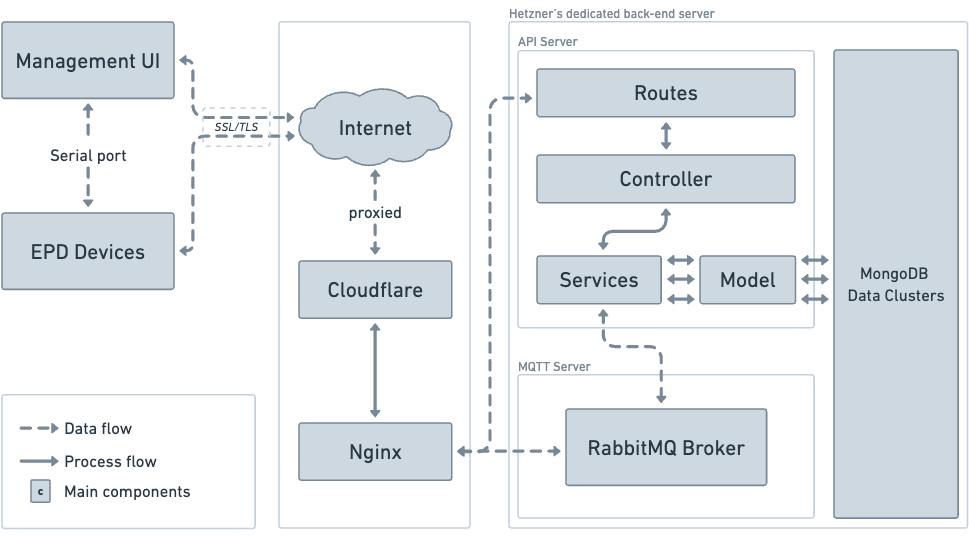
\includegraphics[scale=0.46]{doc/thesis/EN/imgs/overall-architecture.png}
    \caption{Overall architecture of the system}
    \label{fig:Fig1}
\end{figure}

\textbf{Figure \ref{fig:Fig1}} illustrates the system's general architecture and provides an overview of its data flow. The system strategically uses the combination of MVCS (Model-View-Controller-Service) and microservice architectures to take advantage of their unique strengths in specific aspects. This hybrid architecture leverages the benefits of both architectural styles, such as scalability, flexibility, and the ability to use different technologies and patterns within each service.

Microservices architecture is a software development method that structures an application as a collection of loosely coupled services. In this architecture, each service can be developed, deployed, and scaled independently, allowing greater scalability, flexibility, and agility than monolithic architectures, as teams can update or fix individual components without impacting the entire system in case of failure. Thanks to its ability to accommodate the dynamic and distributed natures of IoT applications, microservice architecture is frequently used in various IoT projects. It allows organizations to build more agile and adaptive applications to handle the complex demands of modern business environments.

On the other hand, the Model-View-Controller-Service (MVCS) architecture is an extension of the traditional Model-View-Controller (MVC) pattern. It introduces a service layer sitting between the Controller and the Model, responsible for containing business logic and rules. This layer abstracts complex business operations, allowing Controllers to focus on handling incoming requests and delegating the heavy lifting to Services. This design pattern is well-suited to many web applications, providing a structured and organized approach to developing complex applications and making it easier to manage, maintain, and scale the system over time.

By combining these two architectures, the system is better equipped to handle the dynamic and distributed nature of IoT applications. It also enables organizations to build more agile and adaptive applications to address the complex demands of modern business environments while ensuring scalability, reliability, and seamless communication between different components.

\subsection{Overall design}
The system is divided into independently deployable services, including the API back-end server and MQTT Server. These services communicate via the MQTT protocol, and the MQTT Server also acts as a broker to relay data to the EPD devices (Figure \ref{fig:Fig3}). API server follows the MVCS pattern with three main components: Controllers handling incoming requests and coordinating responses, Services containing the business logic and rules of the application, and Models interacting with the database, managing data storage and retrieval, while Management UI and EPD devices act as a View component (Figure \ref{fig:Fig2}).
\subsubsection{MVCS architecture}
The system has three data types, and the packages of each type handling operation share the same structure: the Controller handles requests about the data type and delegates them to the Service, which processes the requests and uses the Model to interact with the database.
\begin{figure}[H]
    \centering
    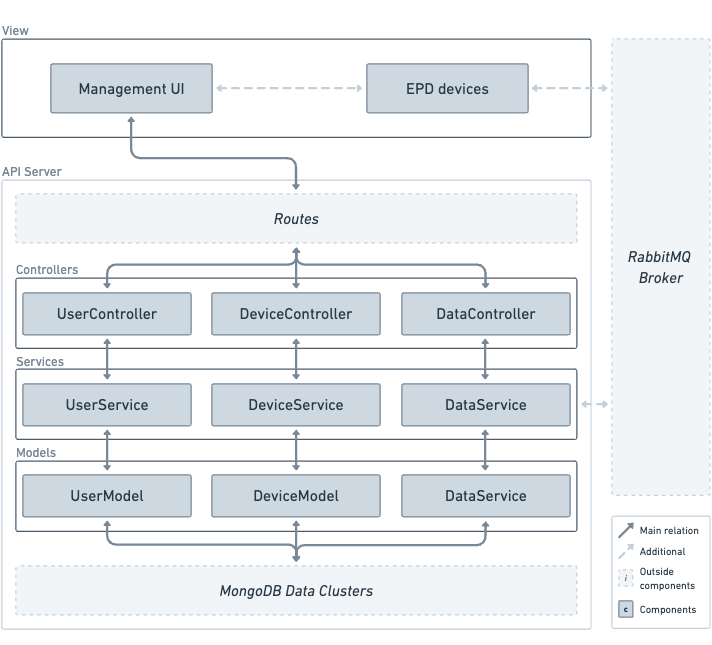
\includegraphics[scale=0.6]{doc/thesis/EN/imgs/api-server.png}
    \caption{MVCS architecture}
    \label{fig:Fig2}
\end{figure}

\subsubsection{MQTT Server}
This service in the system acts as an intermediary, managing the state of all MQTT client connections, subscriptions, and message exchanges.
\begin{figure}[H]
    \centering
    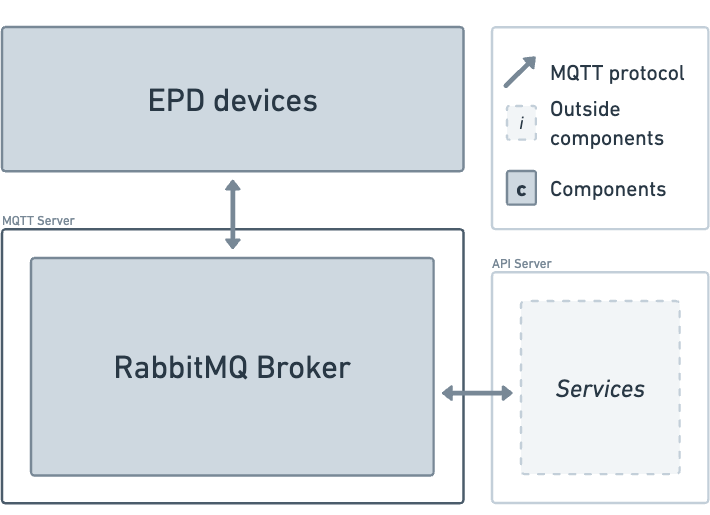
\includegraphics[scale=0.3]{doc/thesis/EN/imgs/mqtt-server.png}
    \caption{MQTT microservice}
    \label{fig:Fig3}
\end{figure}

\subsection{Detailed package design}
\subsubsection{Models}
\begin{figure}[htbp]
    \centering
    \begin{tikzpicture}[]
         \begin{umlpackage}{Models}
            \umlclass[x = 3, y = 8, scale = 0.6]{UserModel}{
                email: string \\
                password: string \\
                name: string \\
                gender: string \\
                \_id: ObjectId \\
                createdAt: time \\
                updatedAt: time
            }{
                \umlvirt{UserModel(userModel: dict): UserModel} \\
                findByIdAndUpdate(id: string): UserModel \\
                findById(id: string): UserModel \\
                findByIdAndRemove(id: string): void \\
                create(data: dict): UserModel \\
                findOne(filter: dict): UserModel
            }

            \umlclass[x = 0, y = 0, scale = 0.6]{DeviceModel}{
                \_id: ObjectId \\
                name: string \\
                ssid: string \\
                pass: string \\
                dataID: ObjectId \\
                dataName: string \\
                active: boolean \\
                createdBy: ObjectId \\
            }{
                \umlvirt{DeviceModel(deviceModel: dict): DeviceModel} \\
                findByIdAndUpdate(id: string): DeviceModel \\
                findById(id: string): DeviceModel \\
                findByIdAndRemove(id: string): void \\
                create(data: dict): DeviceModel \\
                findOne(filter: dict): DeviceModel \\
                find(filter: dict): Array(DeviceModel)
            }
            
            \umlclass[x = 7, y = 0, scale = 0.6]{DataModel}{
                \_id: ObjectId \\
                type: string \\
                name: string \\
                email: string \\
                input2: string \\
                input3: string \\
                input4: string \\
                active: boolean \\
                activeStartTime: uint \\
                deviceID: ObjectId \\
                deviceName: string \\
                activeTimestamp: Array \\
                fontStyle: string \\
                designSchema: string \\
                createdBy: ObjectId
            }{
                \umlvirt{DataModel(deviceModel: dict): DataModel} \\
                findByIdAndUpdate(id: string): DataModel \\
                findById(id: string): DataModel \\
                findByIdAndRemove(id: string): void \\
                findByIdAndDelete(id: string): void \\
                create(data: dict): DataModel \\
                findOne(filter: dict): DataModel
            }
            
            \umlassoc[mult1=1, mult2=*, pos1=0.03, pos2=0.8, align1=left, align2=left]{UserModel}{DeviceModel}
            \umlassoc[mult1=1, mult2=*, pos1=0.03, pos2=0.8, align1=right, align2=right]{UserModel}{DataModel}

            % Bidirectional Dependency
            \umldashedline{DeviceModel}{DataModel}
            \umldep[arg=updates, pos=0.5]{DeviceModel}{DataModel}
            \umldep[pos=0.5]{DataModel}{DeviceModel}
         \end{umlpackage}
    \end{tikzpicture}
    \caption{General use case diagram of the data management system}
    \label{fig:ModelClassDiagram}
\end{figure}

\subsubsection{Services}
\begin{figure}[htbp]
    \centering
    \begin{tikzpicture}[]
         \begin{umlpackage}{Services}
            \umlclass[x = 3, y = 3, scale = 0.6]{UserService}{}{
                findUserByEmail(email: string): UserModel \\
                createUser(user: dict): UserModel \\
                getUserById(id: string): UserModel \\
                updateUser(id: string, user: dict): UserModel \\
            }

            \umlclass[x = 0, y = 0, scale = 0.6]{DeviceService}{}{
                getAllDevices(filter: dict): Array(DeviceModel) \\
                getDeviceById(id: string): DeviceModel \\
                createDevice(data: dict, userId: string): DeviceModel \\
                updateDevice(id: string, data: dict): DeviceModel \\
                deleteDevice(id: string, userId: string): void
            }
            
            \umlclass[x = 6, y = 0, scale = 0.6]{DataService}{}{
                findDataByEmail(email: string): DataModel \\
                getAllData(filter: dict): Array(DataModel) \\
                getDataById(id: string): DataModel \\
                createData(data: dict, userId: string): DataModel \\
                updateData(id: string, data: dict): DataModel \\
                deleteData(id: string, userId: string): void
            }
         \end{umlpackage}
    \end{tikzpicture}
    \caption{General use case diagram of the data management system}
    \label{fig:ServiceClassDiagram}
\end{figure}

\subsubsection{Controllers}
\begin{figure}[htbp]
    \centering
    \begin{tikzpicture}[]
         \begin{umlpackage}{Controllers}
            \umlclass[x = 3, y = 3, scale = 0.6]{UserController}{
                userService: UserService
            }{
                register(): void \\
                login(id: string): void \\
                getAccountById(): UserModel \\
                updateAccount(): UserModel
            }

            \umlclass[x = 0, y = 0, scale = 0.6]{DeviceController}{
                deviceService: DeviceService
            }{
                
                getAllDevices(): Array(DeviceModel) \\
                createDevice(): DeviceModel \\
                getDeviceById(): DeviceModel \\
                updateDevice(): DeviceModel \\
                deleteDevice(): void
            }
            
            \umlclass[x = 5, y = 0, scale = 0.6]{DataController}{
                dataService: DataService
            }{
                getAllData(): Array(DataModel) \\
                createData(): DataModel \\
                getDataById(): DataModel \\
                updateData(): DataModel \\
                deleteData(): void
            }
            
         \end{umlpackage}
    \end{tikzpicture}
    \caption{General use case diagram of the data management system}
    \label{fig:DataClassDiagram}
\end{figure}

\subsubsection{Views}
\begin{figure}[htbp]
    \centering
    \begin{tikzpicture}[]
         \begin{umlpackage}{Views}
            \umlclass[x = -1, y = 3, scale = 0.6]{AccountView}{}{
                handleSubmit(e: event): void \\
            }
            
            \umlclass[x = 2.6, y = 3, scale = 0.6]{NewDeviceView}{}{
                connectESP(): void \\
                handleSubmit(e: event): void \\
                handleReset(): void
            }

            \umlclass[x = 6.2, y = 3, scale = 0.6]{DeviceView}{}{
                connectESP(): void \\
                deleteItem(): void \\
                handleSubmit(e: event): void \\
                handleReset(): void
            }
            
            \umlclass[x = 0, y = 0.7, scale = 0.6]{NewDataView}{}{
                handleStage(e: event): void \\
                handleSubmit(e: event): void \\
                handleReset(): void \\
                getActiveDevices(): Array(DeviceModel)
            }

            \umlclass[x = 5, y = 1, scale = 0.6]{DataView}{}{
                handleSubmit(e: event): void \\
                deleteItem(): void \\
                getActiveDevices(): Array(DeviceModel)
            }
         \end{umlpackage}
    \end{tikzpicture}
    \caption{General use case diagram of the data management system}
    \label{fig:DataClassDiagram}
\end{figure}


\section{Detailed design}
\subsection{User interface design}
The architecture and user interface of this system are meticulously tailored for computer displays, ensuring optimal functionality and visual experience on larger screens. The design is customized to leverage the expansive real estate of computer monitors, facilitating ease of use and comprehensive information display. This focus on computer-targeted design means that the system is not intended for mobile use, and as such, it may not provide an ideal user experience or full functionality on smaller mobile device screens. The decision to specialize in computer displays stems from a commitment to delivering a high-quality, immersive experience that fully utilizes the capabilities and advantages of larger screens typically associated with desktop or laptop computers.
\begin{figure}[H]
    \centering
    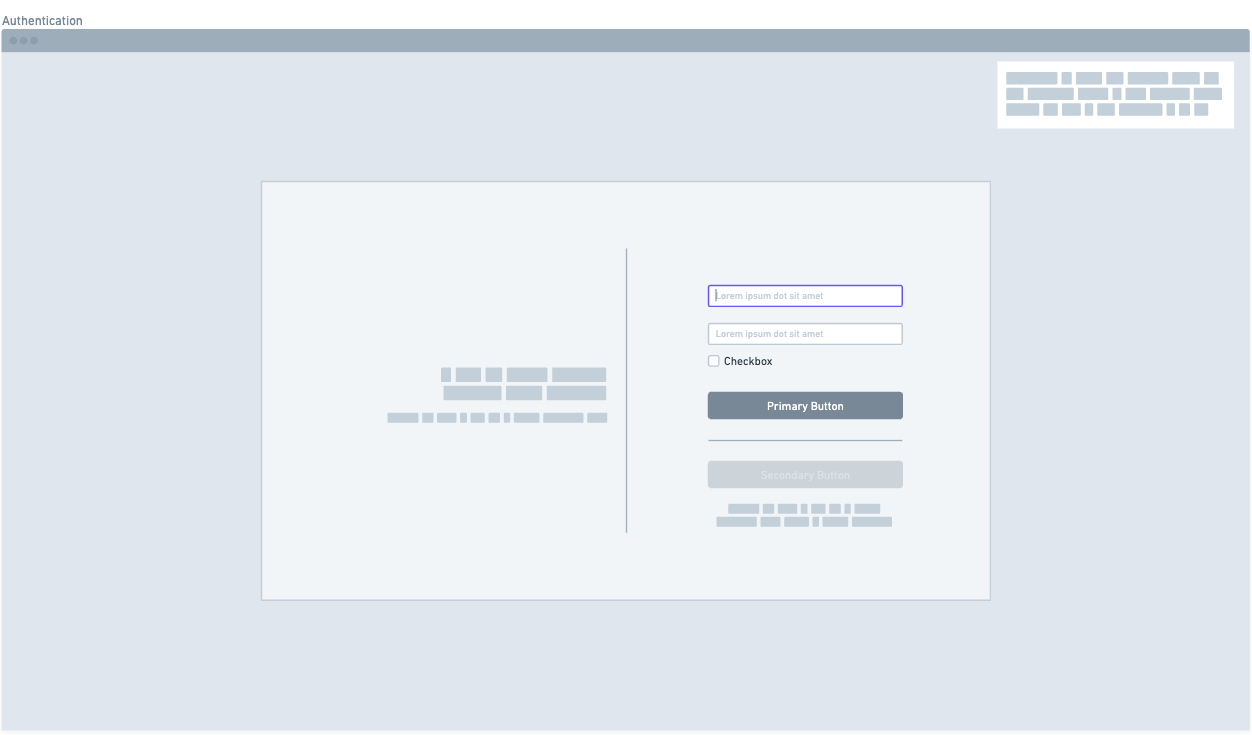
\includegraphics[scale=0.35]{doc/thesis/EN/imgs/mockup1.png}
    \caption{Mockup display of authentication page}
    \label{fig:Mockup1}
\end{figure}
\begin{figure}[H]
    \centering
    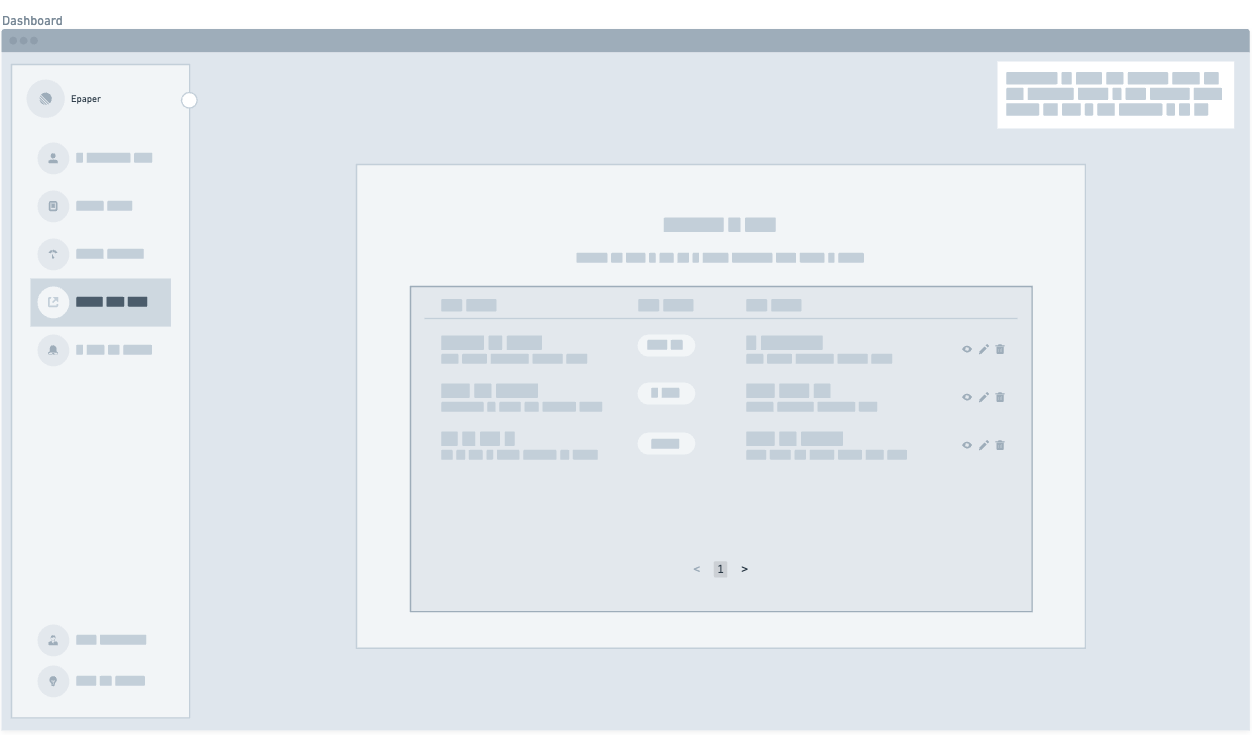
\includegraphics[scale=0.35]{doc/thesis/EN/imgs/mockup2.png}
    \caption{Mockup display of dashboard page}
    \label{fig:Mockup2}
\end{figure}
\begin{figure}[H]
    \centering
    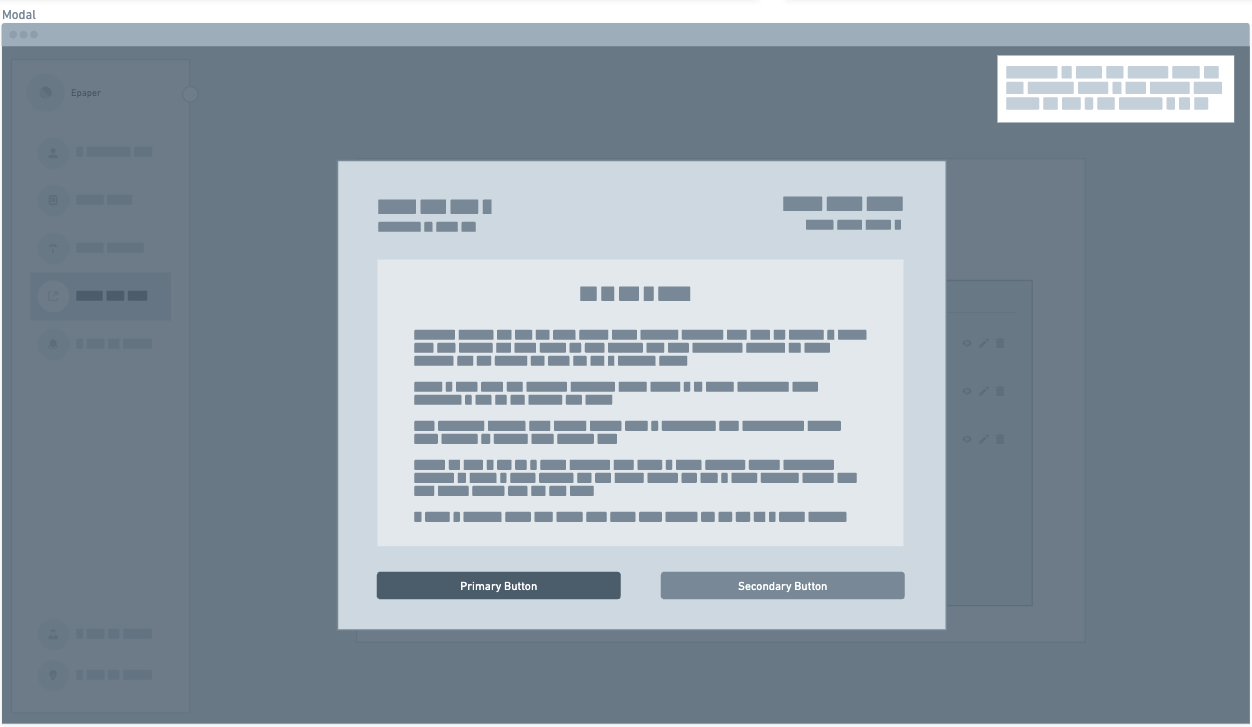
\includegraphics[scale=0.35]{doc/thesis/EN/imgs/mockup3.png}
    \caption{Mockup display of modal component}
    \label{fig:Mockup3}
\end{figure}
\begin{figure}[H]
    \centering
    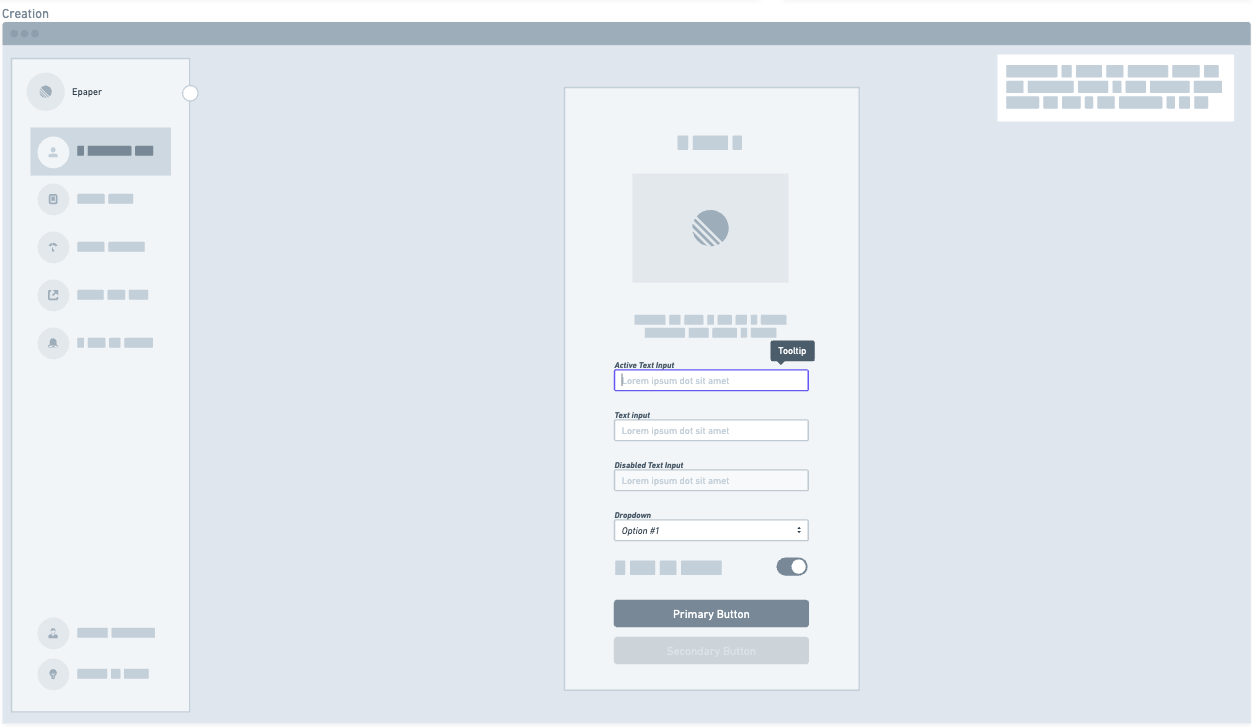
\includegraphics[scale=0.35]{doc/thesis/EN/imgs/mockup4.png}
    \caption{Mockup display of creation page}
    \label{fig:Mockup4}
\end{figure}

\subsection{Layer design}
Each sub-section below demonstrates the workflow of each class participating in each use case in the form of a class diagram and a responding sequence diagram. Each class only shows relevant methods used in the use case.
\subsubsection{Class and sequence diagram of use case "Register a new device"}
\begin{figure}[H]
    \centering
    \begin{tikzpicture}
        % \draw (-1.5, 2.5) rectangle (13, -8);
    
        % Define system boundary
        \umlactor[x = -0.5, y = 4, scale = 0.7]{Manager}
        \umlactor[x = 2, y = 4.5, scale = 0.7]{EPD Devices}
        
        \begin{umlpackage}{pkg}
            \umlclass[x = 0, y = 7, scale = 0.5]{NewDeviceView}{}{
                connectESP(): void \\
                handleSubmit(e: event): void \\
                handleReset(): void
            }
            
            \umlclass[x = 4, y = 7, scale = 0.5]{DeviceController}{
                deviceService: DeviceService
            }{
                createDevice(): DeviceModel
            }

            \umlclass[x = 3, y = 2, scale = 0.5]{DeviceService}{}{
                createDevice(data: dict, userId: string): DeviceModel
            }

            \umlclass[x = 6, y = 4.5, scale = 0.5]{DeviceModel}{
                \_id: ObjectId \\
                name: string \\
                ssid: string \\
                pass: string \\
                dataID: ObjectId \\
                dataName: string \\
                active: boolean \\
                createdBy: ObjectId \\
            }{
                create(data: dict): DeviceModel
            }
        \end{umlpackage}
        
        \umluniassoc[]{Manager}{NewDeviceView}
        \umluniassoc[]{NewDeviceView}{EPD Devices}
        \umluniassoc[]{NewDeviceView}{DeviceController}
        \umluniassoc[]{DeviceController}{DeviceService}
        \umluniassoc[]{DeviceService}{DeviceModel}
    \end{tikzpicture}
    \caption{Detailed use case of Data Management function}
    \label{fig:usecasediagram}
\end{figure}

\begin{figure}[H]
    \centering
    \begin{tikzpicture}[every node/.style={scale=0.8, font=\tiny}]
        \begin{umlseqdiag}
            \umlactor[no ddots, scale = 1.6, x = -1]{Manager}
            \umlactor[no ddots, scale = 1.6, x = 0.5]{EPD Device}
            \umlboundary[no ddots, scale = 1.6, x = 2.7]{NewDeviceView}
            \umlcontrol[no ddots, scale = 1.6, x = 5.2]{DeviceController}
            \umlcontrol[no ddots, scale = 1.6, x = 7.7]{DeviceService}
            \umlentity[no ddots, scale = 1.6, x = 10]{DeviceModel}
            \umlentity[no ddots, scale = 1.6, x = 12]{MQTT Broker}

            \begin{umlcall}[op={Connect ESP device}, dt = 5]{Manager}{NewDeviceView}
                \begin{umlcall}[op={connectESP()}, dt = 5, with return]{NewDeviceView}{EPD Device}
                \end{umlcall}
            \end{umlcall}
            \begin{umlcall}[op={handleSubmit()}, with return]{Manager}{NewDeviceView}
                \begin{umlcall}[op={createDevice()}, return = {device}]{NewDeviceView}{DeviceController}
                    \begin{umlcall}[op={createDevice()}, return = {device}]{DeviceController}{DeviceService}
                        \begin{umlcall}[op={create()}, return = {device}]{DeviceService}{DeviceModel}
                        \end{umlcall}
                        \begin{umlcall}[op={subscribe()}, return = {acknowledge}]{DeviceService}{MQTT Broker}
                        \end{umlcall}
                    \end{umlcall}
                \end{umlcall}
                
                \begin{umlcall}[op={write()}]{NewDeviceView}{EPD Device}
                    \begin{umlcall}[op={subscribe()}, return = {acknowledge}]{EPD Device}{MQTT Broker}
                    \end{umlcall}
                \end{umlcall}
            \end{umlcall}
                
        \end{umlseqdiag}
    \end{tikzpicture}
    \caption{Caption}
    \label{fig:enter-label}
\end{figure}


\subsubsection{Class and sequence diagram of use case "Add a new data"}
\begin{figure}[H]
    \centering
    \begin{tikzpicture}
        % Define system boundary
        \umlactor[x = 3, y = 10, scale = 0.7]{Manager}
        \umlactor[x = 9.5, y = 4, scale = 0.7]{EPD Devices}
        
        \begin{umlpackage}{pkg}
            \umlclass[x = 8, y = 10, scale = 0.5]{NewDataView}{}{
                handleStage(e: event): void \\
                handleSubmit(e: event): void \\
                handleReset(): void \\
                getActiveDevices(): Array(DeviceModel)
            }

            \umlclass[x = 3, y = 7.5, scale = 0.5]{DataController}{
                dataService: DataService
            }{
                createData(): DataModel
            }

            \umlclass[x = 8, y = 7.5, scale = 0.5]{DeviceController}{
                deviceService: DeviceService
            }{
                getAllDevices(): Array(DeviceModel) \\
                updateDevice(): DeviceModel
            }

            \umlclass[x = 5, y = 5, scale = 0.5]{DataService}{}{
                createData(data: dict, userId: string): DataModel
            }

            \umlclass[x = 4, y = 2, scale = 0.5]{DeviceService}{}{
                getAllDevices(filter: dict): Array(DeviceModel)
            }

            \umlclass[x = 14, y = 2, scale = 0.5]{DeviceModel}{
                \_id: ObjectId \\
                name: string \\
                ssid: string \\
                pass: string \\
                dataID: ObjectId \\
                dataName: string \\
                active: boolean \\
                createdBy: ObjectId \\
            }{
                findByIdAndUpdate(id: string): DeviceModel \\
                findById(id: string): DeviceModel \\
                find(filter: dict): Array(DeviceModel)
            }
            
            \umlclass[x = 13, y = 8, scale = 0.5]{DataModel}{
                \_id: ObjectId \\
                type: string \\
                name: string \\
                email: string \\
                input2: string \\
                input3: string \\
                input4: string \\
                active: boolean \\
                activeStartTime: uint \\
                deviceID: ObjectId \\
                deviceName: string \\
                activeTimestamp: Array \\
                fontStyle: string \\
                designSchema: string \\
                createdBy: ObjectId
            }{
                findByIdAndUpdate(id: string): DataModel \\
                findById(id: string): DataModel \\
                create(data: dict): DataModel
            }
        \end{umlpackage}
        
        \umluniassoc[]{Manager}{NewDataView}
        \umluniassoc[geometry = |-, anchor1 = 80, anchor2 = -180]{DataService}{EPD Devices}
        \umluniassoc[geometry = |-, anchor1 = 100, anchor2 = -180]{DeviceService}{EPD Devices}
        \umluniassoc[]{NewDataView}{DataController}
        \umluniassoc[]{NewDataView}{DeviceController}
        \umluniassoc[]{DataController}{DataService}
        \umluniassoc[geometry = |-, anchor1 = -90, anchor2 = 5]{DeviceController}{DeviceService}
        \umluniassoc[geometry = -|, anchor1 = 0, anchor2 = -90]{DataService}{DataModel}
        \umluniassoc[geometry = -|, anchor1 = 0, anchor2 = 90]{DataService}{DeviceModel}
        \umluniassoc[]{DeviceService}{DeviceModel}
    \end{tikzpicture}
    \caption{Detailed use case of Data Management function}
    \label{fig:usecasediagram}
\end{figure}

\begin{figure}[H]
    \centering
    \begin{tikzpicture}[every node/.style={scale=0.7, font=\tiny}]
        \begin{umlseqdiag}
            \umlactor[no ddots, scale = 1.6, x = -1]{Manager}
            \umlactor[no ddots, scale = 1.6, x = 0.5]{EPD Device}
            \umlboundary[no ddots, scale = 1.6, x = 2.7]{NewDataView}
            \umlcontrol[no ddots, scale = 1.6, x = 5.2]{DataController}
            \umlcontrol[no ddots, scale = 1.6, x = 7.7]{DeviceController}
            \umlcontrol[no ddots, scale = 1.6, x = 10]{DataService}
            \umlcontrol[no ddots, scale = 1.6, x = 12]{DeviceService}
            \umlentity[no ddots, scale = 1.6, x = 15]{DataModel}
            \umlentity[no ddots, scale = 1.6, x = 18]{DeviceModel}
            \umlentity[no ddots, scale = 1.6, x = 21]{MQTT Broker}

            \begin{umlcall}[op={Select data type}, dt = 5, with return]{Manager}{NewDataView}
                \begin{umlcall}[op={Show submit form}]{NewDataView}{NewDataView}
                \end{umlcall}
            \end{umlcall}
            
            \begin{umlcall}[op={Fill submit form}, with return]{Manager}{NewDataView}
                \begin{umlcall}[op={Check }]{NewDataView}{NewDataView}
                \end{umlcall}
            \end{umlcall}
            \begin{umlcall}[op={handleSubmit()}, with return]{Manager}{NewDataView}
                \begin{umlcall}[with return]{NewDataView}{DataController}
                    \begin{umlcall}[op={createDevice()}, return = {device}]{DataController}{DataService}
                        \begin{umlcall}[op={createData()}, return = {device}]{DataService}{DataModel}
                            \begin{umlcall}[op={create()}]{DataModel}{DataModel}
                            \end{umlcall}
                        \end{umlcall}
                        \begin{umlcall}[op={subscribe()}, return = {acknowledge}]{DataService}{MQTT Broker}
                        \end{umlcall}
                    \end{umlcall}
                \end{umlcall}
                
                \begin{umlcall}[op={write()}]{NewDataView}{EPD Device}
                    \begin{umlcall}[op={subscribe()}, return = {acknowledge}]{EPD Device}{MQTT Broker}
                    \end{umlcall}
                \end{umlcall}
            \end{umlcall}
                
        \end{umlseqdiag}
    \end{tikzpicture}
    \caption{Caption}
    \label{fig:enter-label}
\end{figure}

\subsubsection{Class and sequence diagram of use case "Change a device information"}
\begin{figure}[H]
    \centering
    \begin{tikzpicture}
        % Define system boundary
        \umlactor[x = 3, y = 10, scale = 0.7]{Manager}
        \umlactor[x = 3, y = 7, scale = 0.7]{EPD Devices}

        \begin{umlpackage}{pkg}
            \umlclass[x = 7, y = 10, scale = 0.5]{DeviceView}{}{
                connectESP(): void \\
                handleSubmit(e: event): void \\
                handleReset(): void
            }

            \umlclass[x = 7, y = 7, scale = 0.5]{DeviceController}{
                deviceService: DeviceService
            }{
                getDeviceById(): DeviceModel \\
                updateDevice(): DeviceModel
            }

            \umlclass[x = 9, y = 4, scale = 0.5]{DeviceService}{}{
                getDeviceById(id: string): DeviceModel \\
                updateDevice(id: string, data: dict): DeviceModel
            }

            \umlclass[x = 3.5, y = 4, scale = 0.5]{DeviceModel}{
                \_id: ObjectId \\
                name: string \\
                ssid: string \\
                pass: string \\
                dataID: ObjectId \\
                dataName: string \\
                active: boolean \\
                createdBy: ObjectId \\
            }{
                findById(id: string): DeviceModel \\
                findByIdAndUpdate(id: string): DeviceModel
            }
            
            \umlclass[x = 11, y = 8, scale = 0.5]{DataModel}{
                \_id: ObjectId \\
                type: string \\
                name: string \\
                email: string \\
                input2: string \\
                input3: string \\
                input4: string \\
                active: boolean \\
                activeStartTime: uint \\
                deviceID: ObjectId \\
                deviceName: string \\
                activeTimestamp: Array \\
                fontStyle: string \\
                designSchema: string \\
                createdBy: ObjectId
            }{
                findByIdAndUpdate(id: string): DataModel \\
                findById(id: string): DataModel
            }
        \end{umlpackage}
        
        \umluniassoc[]{Manager}{DeviceView}
        \umluniassoc[]{DeviceService}{EPD Devices}
        \umluniassoc[]{DeviceView}{EPD Devices}
        \umluniassoc[]{DeviceView}{DeviceController}
        \umluniassoc[]{DeviceController}{DeviceService}
        \umluniassoc[]{DeviceService}{DataModel}
        \umluniassoc[]{DeviceService}{DeviceModel}
    \end{tikzpicture}
    \caption{Detailed use case of Data Management function}
    \label{fig:usecasediagram}
\end{figure}

\subsubsection{Class and sequence diagram of use case "Change data information"}
\begin{figure}[H]
    \centering
    \begin{tikzpicture}
        % Define system boundary
        \umlactor[x = 3, y = 10, scale = 0.7]{Manager}
        \umlactor[x = 9.5, y = 4, scale = 0.7]{EPD Devices}
        
        \begin{umlpackage}{pkg}
            \umlclass[x = 8, y = 10, scale = 0.5]{DataView}{}{
                handleSubmit(e: event): void \\
                getActiveDevices(): Array(DeviceModel)
            }

            \umlclass[x = 3, y = 7.5, scale = 0.5]{DataController}{
                dataService: DataService
            }{
                getDataById(): DataModel \\
                updateData(): DataModel
            }

            \umlclass[x = 8, y = 7.5, scale = 0.5]{DeviceController}{
                deviceService: DeviceService
            }{
                getAllDevices(): Array(DeviceModel) \\
                updateDevice(): DeviceModel
            }

            \umlclass[x = 5, y = 5, scale = 0.5]{DataService}{}{
                getDataById(id: string): DataModel \\
                updateData(id: string, data: dict): DataModel
            }

            \umlclass[x = 4, y = 2, scale = 0.5]{DeviceService}{}{
                getAllDevices(filter: dict): Array(DeviceModel)
            }

            \umlclass[x = 14, y = 2, scale = 0.5]{DeviceModel}{
                \_id: ObjectId \\
                name: string \\
                ssid: string \\
                pass: string \\
                dataID: ObjectId \\
                dataName: string \\
                active: boolean \\
                createdBy: ObjectId \\
            }{
                findByIdAndUpdate(id: string): DeviceModel \\
                findById(id: string): DeviceModel \\
                find(filter: dict): Array(DeviceModel)
            }
            
            \umlclass[x = 13, y = 8, scale = 0.5]{DataModel}{
                \_id: ObjectId \\
                type: string \\
                name: string \\
                email: string \\
                input2: string \\
                input3: string \\
                input4: string \\
                active: boolean \\
                activeStartTime: uint \\
                deviceID: ObjectId \\
                deviceName: string \\
                activeTimestamp: Array \\
                fontStyle: string \\
                designSchema: string \\
                createdBy: ObjectId
            }{
                findByIdAndUpdate(id: string): DataModel \\
                findById(id: string): DataModel \\
            }
        \end{umlpackage}
        
        \umluniassoc[]{Manager}{DataView}
        \umluniassoc[geometry = |-, anchor1 = 80, anchor2 = -180]{DataService}{EPD Devices}
        \umluniassoc[geometry = |-, anchor1 = 100, anchor2 = -180]{DeviceService}{EPD Devices}
        \umluniassoc[]{DataView}{DataController}
        \umluniassoc[]{DataView}{DeviceController}
        \umluniassoc[]{DataController}{DataService}
        \umluniassoc[geometry = |-, anchor1 = -90, anchor2 = 5]{DeviceController}{DeviceService}
        \umluniassoc[geometry = -|, anchor1 = 0, anchor2 = -90]{DataService}{DataModel}
        \umluniassoc[geometry = -|, anchor1 = 0, anchor2 = 90]{DataService}{DeviceModel}
        \umluniassoc[]{DeviceService}{DeviceModel}
    \end{tikzpicture}
    \caption{Detailed use case of Data Management function}
    \label{fig:usecasediagram}
\end{figure}

\subsubsection{Class and sequence diagram of use case "Remove a device"}
\begin{figure}[H]
    \centering
    \begin{tikzpicture}
        % Define system boundary
        \umlactor[x = 3, y = 10, scale = 0.7]{Manager}
        \umlactor[x = 3, y = 7, scale = 0.7]{EPD Devices}

        \begin{umlpackage}{pkg}
            \umlclass[x = 7, y = 10, scale = 0.5]{DeviceView}{}{
                deleteItem(): void
            }

            \umlclass[x = 7, y = 7, scale = 0.5]{DeviceController}{
                deviceService: DeviceService
            }{
                deleteDevice(): void
            }

            \umlclass[x = 9, y = 4, scale = 0.5]{DeviceService}{}{
                getDeviceById(id: string): DeviceModel \\
                deleteDevice(id: string, userId: string): void
            }

            \umlclass[x = 3.5, y = 4, scale = 0.5]{DeviceModel}{
                \_id: ObjectId \\
                name: string \\
                ssid: string \\
                pass: string \\
                dataID: ObjectId \\
                dataName: string \\
                active: boolean \\
                createdBy: ObjectId \\
            }{
                findByIdAndRemove(id: string): void \\
            }
            
            \umlclass[x = 11, y = 8, scale = 0.5]{DataModel}{
                \_id: ObjectId \\
                type: string \\
                name: string \\
                email: string \\
                input2: string \\
                input3: string \\
                input4: string \\
                active: boolean \\
                activeStartTime: uint \\
                deviceID: ObjectId \\
                deviceName: string \\
                activeTimestamp: Array \\
                fontStyle: string \\
                designSchema: string \\
                createdBy: ObjectId
            }{
                findByIdAndUpdate(id: string): DataModel \\
            }
        \end{umlpackage}
        
        \umluniassoc[]{Manager}{DeviceView}
        \umluniassoc[]{DeviceService}{EPD Devices}
        \umluniassoc[]{DeviceView}{EPD Devices}
        \umluniassoc[]{DeviceView}{DeviceController}
        \umluniassoc[]{DeviceController}{DeviceService}
        \umluniassoc[]{DeviceService}{DataModel}
        \umluniassoc[]{DeviceService}{DeviceModel}
    \end{tikzpicture}
    \caption{Detailed use case of Data Management function}
    \label{fig:usecasediagram}
\end{figure}

\subsubsection{Class and sequence diagram of use case "Remove a data"}
\begin{figure}[H]
    \centering
    \begin{tikzpicture}
        % Define system boundary
        \umlactor[x = 3, y = 10, scale = 0.7]{Manager}
        \umlactor[x = 6.5, y = 6.5, scale = 0.7]{EPD Devices}
        
        \begin{umlpackage}{pkg}
            \umlclass[x = 8, y = 10, scale = 0.5]{DataView}{}{
                deleteItem(): void
            }

            \umlclass[x = 4, y = 7.5, scale = 0.5]{DataController}{
                dataService: DataService
            }{
                deleteData(): void
            }

            \umlclass[x = 4, y = 4, scale = 0.5]{DataService}{}{
                getDataById(id: string): DataModel \\
                deleteData(id: string, userId: string): void
            }

            \umlclass[x = 9, y = 2, scale = 0.5]{DeviceModel}{
                \_id: ObjectId \\
                name: string \\
                ssid: string \\
                pass: string \\
                dataID: ObjectId \\
                dataName: string \\
                active: boolean \\
                createdBy: ObjectId \\
            }{
                findByIdAndUpdate(id: string): DeviceModel \\
                findById(id: string): DeviceModel
            }
            
            \umlclass[x = 10, y = 6.5, scale = 0.5]{DataModel}{
                \_id: ObjectId \\
                type: string \\
                name: string \\
                email: string \\
                input2: string \\
                input3: string \\
                input4: string \\
                active: boolean \\
                activeStartTime: uint \\
                deviceID: ObjectId \\
                deviceName: string \\
                activeTimestamp: Array \\
                fontStyle: string \\
                designSchema: string \\
                createdBy: ObjectId
            }{
                findById(id: string): DataModel \\
                findByIdAndDelete(id: string): void
            }
        \end{umlpackage}
        
        \umluniassoc[]{Manager}{DataView}
        \umluniassoc[geometry = |-, anchor1 = 70, anchor2 = -180]{DataService}{EPD Devices}
        \umluniassoc[]{DataView}{DataController}
        \umluniassoc[]{DataController}{DataService}
        \umluniassoc[]{DataService}{DataModel}
        \umluniassoc[geometry = |-, anchor1 = -90, anchor2 = -180]{DataService}{DeviceModel}
    \end{tikzpicture}
    \caption{Detailed use case of Data Management function}
    \label{fig:usecasediagram}
\end{figure}

\subsubsection{Class and sequence diagram of use case "Register new account"}
    \begin{landscape}

\begin{figure}[H]
    \centering
    \begin{tikzpicture}
        % Define system boundary
        \umlactor[x = 1, y = 10, scale = 0.7]{Manager}
        \umlactor[x = 8, y = 10, scale = 0.7]{Administrator}
        
        \begin{umlpackage}{pkg}
            \umlclass[x = 4.5, y = 10, scale = 0.6]{AccountView}{}{
                handleSubmit(e: event): void
            }

            \umlclass[x = 1, y = 7, scale = 0.6]{UserController}{
                userService: UserService
            }{
                register(): void \\
            }

            \umlclass[x = 7, y = 7, scale = 0.6]{UserService}{}{
                findUserByEmail(email: string): UserModel \\
                createUser(user: dict): UserModel
            }

            \umlclass[x = 3, y = 4, scale = 0.6]{UserModel}{
                email: string \\
                password: string \\
                name: string \\
                gender: string \\
                \_id: ObjectId \\
                createdAt: time \\
                updatedAt: time
            }{
                create(data: dict): UserModel \\
                findOne(filter: dict): UserModel
            }
        \end{umlpackage}
        
        \umluniassoc[]{Manager}{AccountView}
        \umluniassoc[]{Administrator}{AccountView}
        \umluniassoc[]{AccountView}{UserController}
        \umluniassoc[]{UserController}{UserService}
        \umluniassoc[]{UserService}{UserModel}
    \end{tikzpicture}
    \caption{Detailed use case of Data Management function}
    \label{fig:usecasediagram}
\end{figure}

\begin{figure}[H]
    \centering
        \begin{tikzpicture}[every node/.style={font=\tiny}]
        \begin{umlseqdiag}
            \umlactor[no ddots, scale = 1.6, x = -1]{Manager/ Administrator}
            \umlboundary[no ddots, scale = 1.6, x = 2]{AccountView}
            \umlcontrol[no ddots, scale = 1.6, x = 4.5]{UserController}
            \umlcontrol[no ddots, scale = 1.6, x = 7.5]{UserService}
            \umlentity[no ddots, scale = 1.6, x = 10]{UserModel}

            \begin{umlcall}[op={HandleSubmit(): void}, dt = 5]{Manager/ Administrator}{AccountView}
                \begin{umlcall}[op={register(): void}, dt = 5]{AccountView}{UserController}

                    \begin{umlcall}[op={findUserByEmail(): void}, dt = 5, return = {user}]{UserController}{UserService}
                        \begin{umlcall}[op={findOne(): UserModel}, dt = 5, return = {user}]{UserService}{UserModel}
                        \end{umlcall}
                    \end{umlcall}
                
                \begin{umlfragment}[type=alt, label={user is null}, inner xsep = 15]
                    \begin{umlcall}[op={success},  type=return, padding = -2]{UserController}{AccountView}
                    \end{umlcall}

                    \begin{umlcall}[op={success},  type=return, dt = 3]{AccountView}{Manager/ Administrator}
                    \end{umlcall}

                    \umlfpart[user existed]
                    \begin{umlcall}[op={email has been used},  type=return]{UserController}{AccountView}
                    \end{umlcall}

                    \begin{umlcall}[op={success},  type=return, dt=3]{AccountView}{Manager/ Administrator}
                    \end{umlcall}
                \end{umlfragment}
                
                \end{umlcall}
            \end{umlcall}
                
        \end{umlseqdiag}
    \end{tikzpicture}
    
    \caption{Caption}
    \label{fig:enter-label}
\end{figure}
    \end{landscape}

\subsubsection{Class and sequence diagram of use case "Sign in"}
\begin{figure}[H]
    \centering
    \begin{tikzpicture}
        % Define system boundary
        \umlactor[x = 1, y = 10, scale = 0.7]{Manager}
        \umlactor[x = 8, y = 10, scale = 0.7]{Administrator}
        
        \begin{umlpackage}{pkg}
            \umlclass[x = 4.5, y = 10, scale = 0.6]{AccountView}{}{
                handleSubmit(e: event): void
            }

            \umlclass[x = 1, y = 7, scale = 0.6]{UserController}{
                userService: UserService
            }{
                login(): void \\
            }

            \umlclass[x = 7, y = 7, scale = 0.6]{UserService}{}{
                findUserByEmail(email: string): UserModel
            }

            \umlclass[x = 3, y = 4, scale = 0.6]{UserModel}{
                email: string \\
                password: string \\
                name: string \\
                gender: string \\
                \_id: ObjectId \\
                createdAt: time \\
                updatedAt: time
            }{
                findOne(filter: dict): UserModel
            }
        \end{umlpackage}
        
        \umluniassoc[]{Manager}{AccountView}
        \umluniassoc[]{Administrator}{AccountView}
        \umluniassoc[]{AccountView}{UserController}
        \umluniassoc[]{UserController}{UserService}
        \umluniassoc[]{UserService}{UserModel}
    \end{tikzpicture}
    \caption{Detailed use case of Data Management function}
    \label{fig:usecasediagram}
\end{figure}

\subsection{Database design}
Phần này có độ dài từ hai đến bốn trang. Sinh viên thiết kế, vẽ và giải thích biểu đồ thực thể liên kết (E-R diagram). Từ đó, sinh viên thiết kế cơ sở dữ liệu tùy theo hệ quản trị cơ sở dữ liệu mà mình sử dụng (SQL, NoSQL, Firebase, v.v.)

\subsubsection{Entity-Relationship diagram}
\begin{figure}[H]
    \centering
    \begin{tikzpicture}[every node/.style={scale=0.8, font=\small}]
        \pic{entity={User}{User}{%
            email \\
            password \\
            name \\
            gender \\
            \_id \\
            createdAt \\
            updatedAt
        }};
        \pic[below=6em of User]{entity={Device}{Device}{%
            \_id \\
            name \\
            ssid \\
            pass \\
            dataID \\
            dataName \\
            active \\
            createdBy                
        }};
        \pic[right=6em of User] {entity={Data}{Data}{%
            \_id \\
            type \\
            name \\
            email \\
            input2 \\
            input3 \\
            input4 \\
            active \\
            activeStartTime \\
            deviceID \\
            deviceName \\
            activeTimestamp \\
            fontStyle \\
            designSchema \\
            createdBy
        }};
        
        \draw[one to omany] (Device.north) -- (User.south);
        \draw[one to omany] (Data.west) -- (User.east);
        \draw[one to oone] (Device.east) -| (Data.south);
    \end{tikzpicture}
\end{figure}

\subsubsection{Detail database design}
{\fontsize{8pt}{8pt}\selectfont 
    \newcolumntype{M}[1]{>{\centering\arraybackslash}m{#1}}
    \newcolumntype{L}[1]{>{\raggedright\arraybackslash}p{#1}}
    \renewcommand{\arraystretch}{2} % Adjust for row height
    \begin{longtable}{ | M{2cm} | L{2cm} | L{1.5cm} | M{1cm} | L{6cm} | }
        \hline
        \textbf{Collection} & \textbf{Field Name} & \textbf{Field Type} & \textbf{Required} & \textbf{Description} \\ 
        \endfirsthead
        \hline
        \textbf{Collection} & \textbf{Field Name} & \textbf{Field Type} & \textbf{Required} & \textbf{Description} \\ 
        \hline
        \endhead
        
        \hline
        \multirow{7}{*}{User}   & \_id              & ObjectId  & * & User's ID used in the system                          \\ \cline{2-5}
                                & email             & String    & * & User's personal email                                 \\ \cline{2-5}
                                & password          & String    & * & Encrypted password of user's account                  \\ \cline{2-5}
                                & name              & String    & * & User's name                                           \\ \cline{2-5}
                                & gender            & String    &   & User's gender                                         \\ \cline{2-5}
                                & createdAt         & Time      & * & Time of account creation                              \\ \cline{2-5}
                                & updatedAt         & Time      & * & Last account update time                              \\
    
        \hline
        \multirow{15}{*}{Data}  & \_id              & ObjectId  & * & Data's ID used in the system                          \\ \cline{2-5}
                                & type              & String    & * & Data type                                             \\ \cline{2-5}
                                & name              & String    & * & Data name                                             \\ \cline{2-5}
                                & email             & String    &   & First information: email                              \\ \cline{2-5}
                                & input2            & String    &   & Second information                                    \\ \cline{2-5}
                                & input3            & String    &   & Third information                                     \\ \cline{2-5}
                                & input4            & String    &   & Fourth information                                    \\ \cline{2-5}
                                & active            & boolean   & * & Display status on EPD device                          \\ \cline{2-5}
                                & activeStartTime   & uint      & * & The display start time                                \\ \cline{2-5}
                                & deviceID          & ObjectId  &   & ID of displayed device                                \\ \cline{2-5}
                                & deviceName        & String    &   & Name of the displayed device                          \\ \cline{2-5}
                                & activeTimestamp   & Array     & * & A list of display time range                          \\ \cline{2-5}
                                & fontStyle         & String    &   & Custom display font style                             \\ \cline{2-5}
                                & designSchema      & String    &   & Custom display theme                                  \\ \cline{2-5}
                                & createdBy         & ObjectId  & * & ID of the user creating the data                      \\
    
        \hline
        \multirow{8}{*}{Device} & \_id              & ObjectId  & * & Device's ID used in the system                        \\ \cline{2-5}
                                & name              & String    &   & Device name                                           \\ \cline{2-5}
                                & ssid              & String    & * & SSID of the network the device is connecting to       \\ \cline{2-5}
                                & pass              & String    & * & Password of the network the device is connecting to   \\ \cline{2-5}
                                & dataID            & ObjectId  &   & ID of displayed data on the device                    \\ \cline{2-5}
                                & dataName          & String    &   & Name of displayed data on the device                  \\ \cline{2-5}
                                & active            & boolean   & * & Connection status of device                           \\ \cline{2-5}
                                & createdBy         & ObjectId  & * & ID of the user creating the data                      \\
                        
        \hline
        \caption{Your Table Caption}
        \label{table:your_table_label}
    \end{longtable}
}
\section{Application Building}
\subsection{Libraries and Tools}
In the development of this project, a suite of sophisticated tools was employed to ensure efficiency and quality in the coding process. Central to this toolkit was Visual Studio Code (VS Code), a versatile and powerful code editor known for its user-friendly interface and wide range of extensions. Alongside VS Code, a variety of other tools were integral to the workflow, such as Mongo Compass to manage the MongoDB database and PlatformIO to work with ESP devices. These also included version control systems for tracking changes and collaborating with team members, debugging tools for identifying and resolving issues, and project management software to keep the development process streamlined and on schedule. Table \ref{fig:table_tools} below lists all the tools and applications used during the development process and also the systems used in the project.

\begin{table}[H]
    \newcolumntype{M}[1]{>{\centering\arraybackslash}m{#1}}
    \newcolumntype{L}[1]{>{\raggedright\arraybackslash}p{#1}}
    \renewcommand{\arraystretch}{2} % Adjust for row height
    \centering{}
    \fontsize{7pt}{8pt}\selectfont 
    \begin{tabular}{| m{3cm} | m{1cm} | m{1.4cm} | m{4cm} | m{4cm} |}
        \hline
        \textbf{Tools used}                     & \textbf{Type} & \textbf{Version}  & \textbf{Description}                                              & \textbf{URL}                                                      \\ \hline
        Visual Studio Code - Insiders (VSCode)  & Tools         & 1.86.0-insider    & Main development environment                                      & \url{https://code.visualstudio.com/insiders}                      \\ \hline
        PlatformIO                              & VSCode Plugins& v3.3.2            & A development ecosystem for embedded and IoT applications         & \url{https://platformio.org}                                      \\ \hline
        Remote Development                      & VSCode Plugins& v0.4.1            & A plugin allowing VSCode to develop on remote systems             & \url{https://code.visualstudio.com/docs/remote/remote-overview}   \\ \hline
        Wokwi Simulator                         & VSCode Plugins& v2.3.2            & Simulator for Embedded \& IoT Systems                             & \url{https://wokwi.com}                                           \\ \hline
        NodeJS                                  & Language      & v20.9.0           & A JavaScript runtime for building scalable network applications   & \url{https://nodejs.org}                                          \\ \hline
        Next.JS                                 & Framework     & v13.4.5           & A framework for server-side rendered React applications           & \url{https://nextjs.org}                                          \\ \hline
        TailwindCSS                             & Framework     & v3.3.2            & A utility-first CSS framework for rapid UI development            & \url{https://tailwindcss.com}                                     \\ \hline
        Express.JS                              & Framework     & v4.18.2           & A web application framework for Node.js                           & \url{https://expressjs.com}                                       \\ \hline
        Mongoose                                & Library       & v8.0.0            & A library for MongoDB and Node.js data modeling                   & \url{https://mongoosejs.com}                                      \\ \hline
        MQTT NPM Package (mqtt)                 & Library       & v5.3.0            & A library for implementing MQTT protocol in Node.js               & \url{https://www.npmjs.com/package/mqtt}                          \\ \hline
        WaveShare EPD Library                   & Library       & v1.0              & A library for interfacing with e-paper displays                   &                                                                   \\ \hline
        Node Version Manager (nvm)              & Tools         & v0.39.2           & A tool for managing multiple Node.js versions                     & \url{https://github.com/nvm-sh/nvm}                               \\ \hline
        Node Package Manager (npm)              & Tools         & v10.1.0           & A package manager managing dependencies in Node.js projects       & \url{https://www.npmjs.com}                                       \\ \hline
        MongoDB Community Edition for Linux     & Tools         & v7.0.2            & An open-source document database for Linux systems                & \url{https://www.mongodb.com/try/download/community}              \\ \hline
        MongoDB Compass                         & Tools         & v1.40.4           & A GUI for MongoDB, simplifying data visualization and management  & \url{https://www.mongodb.com/products/compass}                    \\ \hline
        RabbitMQ                                & Tools         & v3.12.10          & An open-source message broker software                            & \url{https://www.rabbitmq.com}                                    \\ \hline
        ESP32 C3-Supermini                      & Device        &                   & A compact microcontroller module for EPD devices                  &                                                                   \\ \hline
        WeAct Studio E-paper 2.9inch display    & Device        &                   & A low-power display module for high-contrast, readable content    & \url{https://www.weact-tc.cn}                                     \\ \hline
        Ubuntu Server                           & System        &                   & A dedicated server in Hetzner, for Web hosting and MQTT Broker    & \url{https://www.hetzner.com}                                     \\ \hline
        Nginx                                   & Tools         & nginx/1.24.0      & A high-performance web server and reverse proxy                   & \url{https://nginx.org}                                           \\ \hline
        Cloudflare                              & Tools         &                   & A service for website performance optimization and security       & \url{https://www.cloudflare.com}                                  \\ \hline
    \end{tabular}
    \caption{Danh sách thư viện và công cụ sử dụng}
    \label{fig:table_tools}
\end{table}

\subsection{Achievement}
Sinh viên trước tiên mô tả kết quả đạt được của mình là gì, ví dụ như các sản phẩm được đóng gói là gì, bao gồm những thành phần nào, ý nghĩa, vai trò?

Sinh viên cần thống kê các thông tin về ứng dụng của mình như: số dòng code, số lớp, số gói, dung lượng toàn bộ mã nguồn, dung lượng của từng sản phẩm đóng gói, v.v. Tương tự như phần liệt kê về công cụ sử dụng, sinh viên cũng nên dùng bảng để mô tả phần thông tin thống kê này.

With the help of tools and libraries in the table \ref{fig:table_tools} above, the project has reached significant milestones and also released a minimum viable product (MVP) including the Management UI, the back-end server, and a couple of EPD devices that can be implemented in many small business environments. While having some minor performance issues, this MVP still proved its usefulness in various use cases, such as mini-markets, schools, and offices, unveiling the enormous potential of the system in a broader spectrum of the service industry.

The whole system is running on the website so the users don't need to install any additional applications. Also, the users just need to plug the EPD device into the computer via a USB port when needed without additional drivers, and the website will automatically recognize the device. Details of the running system are shown in the table below

\begin{table}[H]
    \newcolumntype{M}[1]{>{\centering\arraybackslash}m{#1}}
    \newcolumntype{L}[1]{>{\raggedright\arraybackslash}p{#1}}
    \renewcommand{\arraystretch}{2} % Adjust for row height
    \centering{}
    \fontsize{7pt}{8pt}\selectfont 
    \begin{tabular}{| m{4cm} | m{6cm} |}
        \hline
        \textbf{Description}    & \textbf{URL}                                          \\ \hline
        Management UI           & \url{https://epaper.artsakh.ventures}                 \\ \hline
        MongoDB Databases       & \url{mongodb://epaper.artsakh.ventures:27017}         \\ \hline
        Back-end server         & \url{https://epaper.artsakh.ventures/api}             \\ \hline
        MQTT Broker             & \url{mqtts://mqtt.epaper.artsakh.ventures}            \\ \hline
        MQTT Management UI      & \url{https://mqtt.epaper.artsakh.ventures/dashboard}  \\ \hline
    \end{tabular}
    \caption{Danh sách thư viện và công cụ sử dụng}
    \label{fig:table_tools}
\end{table}

\subsection{Illustration of main functions}
To manage EPD Devices and data, users need to log in with credentials as illustrated in the picture \ref{}. After logging in, the user can choose to create data/device or go to the dashboard to view from the sidebar on the left. 

When creating data/device, the user can easily follow on-screen instructions and fill in the required information. All the steps are annotated in detail, and the rendered display is showing in real-time, which helps improve user experience. 

The EPD Device connects to MQTT Broker and subscribe to its ID as topic. The left side of the picture \ref{} belows indicates the device display when no data is stored, and the right side show the device display when a data is stored in the device. The d
evice is running on battery, which can last for 5 - 6 hours before needing to recharge. in the scope of the project, this is still reasonable and acceptable as the product is still in the prototype stage, and not optimized for higher endurance in a real-life environment. 

\section{Testing}
Phần này có độ dài từ hai đến ba trang. Sinh viên thiết kế các trường hợp kiểm thử cho hai đến ba chức năng quan trọng nhất. Sinh viên cần chỉ rõ các kỹ thuật kiểm thử đã sử dụng. Chi tiết các trường hợp kiểm thử khác, nếu muốn trình bày, sinh viên đưa vào phần phụ lục.
Sinh viên sau cùng tổng kết về số lượng các trường hợp kiểm thử và kết quả kiểm thử. Sinh viên cần phân tích lý do nếu kết quả kiểm thử không đạt.

\section{Deployment}
\subsection{CI/CD}
 All of the project's source code is hosted and managed on Github, using Continuous Integration and Continuous Delivery (CI/CD) to automate the deployment. When a new commit on main branch is created, a workflow is triggered to update both front-end and back-end in the hosting server. Detail and the log of the workflow can be monitored in Action setion in .

 \subsection{Servers}

The system uses two dedicated servers both running on Ubuntu 20.04 Jammy, with detail nand purpose are listed in the table below:
\begin{table}[H]
    \newcolumntype{M}[1]{>{\centering\arraybackslash}m{#1}}
    \newcolumntype{L}[1]{>{\raggedright\arraybackslash}p{#1}}
    \renewcommand{\arraystretch}{2} % Adjust for row height
    \centering{}
    \fontsize{7pt}{8pt}\selectfont 
    \begin{tabular}{| m(4cm) | m{4cm} | m{6cm} |}
        \hline
                   j         & \textbf{Back-end Server (web-server)} & \textbf{MQTT Broker (laboratory)} \\ \hline
        IP address          & 65.108.79.164                         & 95.217.121.243                    \\ \hline
        Operating System    & Ubuntu 20.04 LTS Jammy                & Ubuntu 20.04 LTS Jammy            \\ \hline
        CPU                 & Intel                                 & Intel                             \\ \hline
        RAM                 & 64GB                                  & 64GB                              \\ \hline
        Storage             & 4TB                                   & 2TB                               \\ \hline
        Service used        & Nginx, MongoDB, ManagementUI, Back-end, OpenSSL & Nginx, RabbitMQ, OpenSSL\\ \hline
    \end{tabular}
    \caption{Danh sách thư viện và công cụ sử dụng}
    \label{fig:table_tools}
\end{table}

At "web-server" server, Management UI and API server are configured as system daemon, with two service files defined in epaper.service and epaper-backend.service. 

\subsection{EPD Devices}

Sinh viên trình bày mô hình và/hoặc cách thức triển khai thử nghiệm/thực tế. Ứng dụng của sinh viên được triển khai trên server/thiết bị gì, cấu hình như thế nào. Kết quả triển khai thử nghiệm nếu có (số lượng người dùng, số lượng truy cập, thời gian phản hồi, phản hồi người dùng, khả năng chịu tải, các thống kê, v.v.)

\end{document}
